\documentclass{article}
\usepackage{graphicx}
\usepackage{url}
\usepackage{tikz} 
\usepackage{amsmath}
\usepackage{makeidx}
\usepackage{amssymb}
\usetikzlibrary{shapes.geometric,  shapes.misc, arrows.meta, positioning}


\title{Market power in an interbank model}
\author{Hector Castillo}
\date{3rd March 2026}

\makeindex

\begin{document}


\maketitle


\subsection*{Balance sheet}

Following model presented in \cite{Delliggatti2024} and \cite{BRINI2023}, We examine a sequential economy that unfolds in discrete time periods, denoted as 
\( t = \{0, 1, 2, \ldots, T\} \). At each point in time \( t =  \{0, 1, 2, \ldots, T\} \), the system consists of \( N \)  banks \( i, j \in \Omega = \{1, \ldots, N\} \). These financial institutions are linked through the credit relationships captured by the set \( V_t \), whose elements represent ordered pairs of distinct banks. Together, banks (nodes or vertices) and their credit links (edges) constitute the 
interbank network \( G_t = (\Omega, V_t) \). The daily balance sheet composition of each bank is specified as follows:
\begin{equation}
\underbrace{L^i_t + C^i_t+ R^i_t}_{\text{assets}}= \underbrace{D^i_t+ E^i_t}_{\text{liabilities}}
\end{equation}

Assets are on the left side and liabilities are on the right side. In particular, \emph{L, C}, and \emph{R} represent long-term assets, liquidity, and reserves, while \emph{D} and \emph{E}
deposits and bank equity $i$ at time $t$. Reserves are a deposit rate that replicates the central bank regulation that sets the minimum amount that a bank should hold in liquid assets ($R^i_t=\hat{r}D^i_t$), which is used in this model $\hat{r}=0.02$.

At every time $t$, deposits are exogenously shocked, and the balance sheet modifies accordingly. Specifically, deposits evolve as
\begin{equation}
\label{evolution_d}
D^i_t = D^i_{t-1} [ \mu + \omega U(0,1)]
\end{equation}

where $U(0,1)$ is a uniformly distributed noise between 0 and 1 and $\mu$ and $\omega$ represent the expected number of negative shocks and thus different market conditions.
This setup achieves stock-flow equilibrium on average, enabling roughly half of market actors to recoup erosion from negative shocks. While not all strict consistency conditions hold, tests confirm that at $\mu=0.7$ and $\omega=0.55$, assets match liabilities per bank, yielding a system-wide balance sheet of zero, as \cite{BRINI2023} demonstrate.

Banks that suffer an increase in deposits or a small negative shock covered with their own capital become potential creditors to the system, with a supply of liquidity denoted as $s^i_t=\Delta D^i_t + C^i_t$. Those loans are obtained by the banks with a negative change in deposits when $\Delta D^i_t + C^i_t \leq 0$. The demand of liquidity of each borrower is $d^i_t=|\Delta D^i_t + C^i_t |$.

In each $t$ the number of borrowers and lenders are not equalized, as our mechanism \ref{evolution_d} is Non-Walrasian. That disequilibrium generates a rationed market increased by the limitation to an only one lender for each borrower, using a mechanism of attachment of lenders and borrowers explained in the next section \ref{attachment_mechanism}.  

As not all borrowers will obtain their full demand for loan $d^i_t$, we define the real loan obtained for a generic borrower $j$ by its lender $i$ as $l^{i,j}_t=min(s^i_t,d^j_t)$. The last resort option for the borrower to obtain the amount of money not covered by the loan is to fire sale its long term assets at $\rho$ price, with a reduction in $L$ of $\nabla L^j_t=\frac{d^j_t-s^i_t}{\rho}$.

\subsection*{Mechanism of attachment of lending agreements}
\label{attachment_mechanism}
At the beginning of each day, agents meet in the interbank market and sign bilateral potential lending
agreements representing the directed links $(i, j) \in V_t$. These agreements can be interpreted as credit lines, which are valid during $t$, and can be used at the request of the borrower $j$ in
case of the lender $i$ available liquidity. The set of all potential lending agreements reproduces the potential interbank network and we explicitly limit to one only possible lender for each borrower, so if we represent as a directed graph where nodes are banks and a incoming link in node $j$ from node $i$ represents the potential lending agreement from creditor $i$ for debtor $j$. The grade of outcoming links is limited to 1, so only one possible potential lender is available.


The preferential lending agreements are determined in each step using a network topology of an Erdös–Rényi random graph $G(N,p_a)$, constructed by connecting initially undirected labeled nodes randomly. 
The nodes $N$ are the banks. Each undirected edge is included in the graph with a parameter of probability $p_a$ without any dependency of previous edges, iterating over each combination of possible distinct nodes $(i,j)$ and after a Bernoulli process with probability $p_a$ we add or not the edge connecting nodes $i$ and $j$:

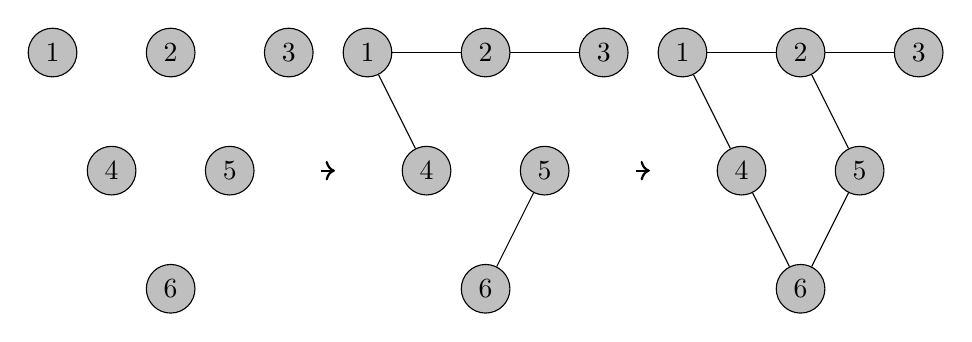
\begin{tikzpicture}[
  node distance=1cm,
  every node/.style={circle, draw, minimum size=0.5cm, fill=lightgray},
  edge/.style={--, thick}
]

% STEP 1: Only nodes
\begin{scope}[local bounding box=step1]
  \node (1a) at (0, 0) {1};
  \node (2a) at (1.5, 0) {2};
  \node (3a) at (3, 0) {3};
  \node (4a) at (0.75, -1.5) {4};
  \node (5a) at (2.25, -1.5) {5};
  \node (6a) at (1.5, -3) {6};
\end{scope}

% STEP 2: Bernoulli process (some edges)
\begin{scope}[local bounding box=step2, xshift=4cm]
  \node (1b) at (0, 0) {1};
  \node (2b) at (1.5, 0) {2};
  \node (3b) at (3, 0) {3};
  \node (4b) at (0.75, -1.5) {4};
  \node (5b) at (2.25, -1.5) {5};
  \node (6b) at (1.5, -3) {6};
  
  \draw (1b) -- (2b);
  \draw (2b) -- (3b);
  \draw (1b) -- (4b);
  \draw (5b) -- (6b);
\end{scope}

% STEP 3: Final random graph
\begin{scope}[local bounding box=step3, xshift=8cm]
  \node (1c) at (0, 0) {1};
  \node (2c) at (1.5, 0) {2};
  \node (3c) at (3, 0) {3};
  \node (4c) at (0.75, -1.5) {4};
  \node (5c) at (2.25, -1.5) {5};
  \node (6c) at (1.5, -3) {6};
  
  \draw (1c) -- (2c);
  \draw (2c) -- (3c);
  \draw (1c) -- (4c);
  \draw (2c) -- (5c);
  \draw (4c) -- (6c);
  \draw (5c) -- (6c);
\end{scope}

% Arrows between steps
\draw[->, thick, shorten >=3pt, shorten <=3pt] (step1.east) -- (step2.west);
\draw[->, thick, shorten >=3pt, shorten <=3pt] (step2.east) -- (step3.west);

\end{tikzpicture}

After the graph is generated, each bank $i$ has $L_i$ connections on the graph, or maybe none, as picture \ref{fig:no_directions} denotes:

\begin{figure}
    \centering
    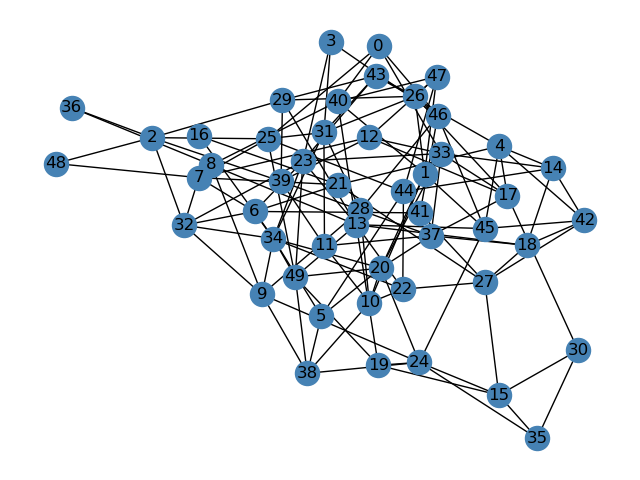
\includegraphics[width=0.5\linewidth]{without_directions.png}
    \caption{Erdös–Rényi without directions with fifty banks}
    \label{fig:no_directions}
\end{figure}

The direction of the connections between nodes (banks) is randomly chosen just after the shock to have one lender or no lender (because each borrower can have only one loan). If there are multiple lenders, we randomly choose one of them and set up the loan for this step. When the current time $t$ is complete, before starting $t+1$ a new graph is generated. The different color in \ref{fig:with_directions} of bank 43 is used to denote the one with more incoming links (more active borrowers). As $p_a=0.1$ there are no isolated banks. Also, the main facts about the network created is added to the graph (such as the Giant Component Size and the number of communities).

\begin{figure}
    \centering
    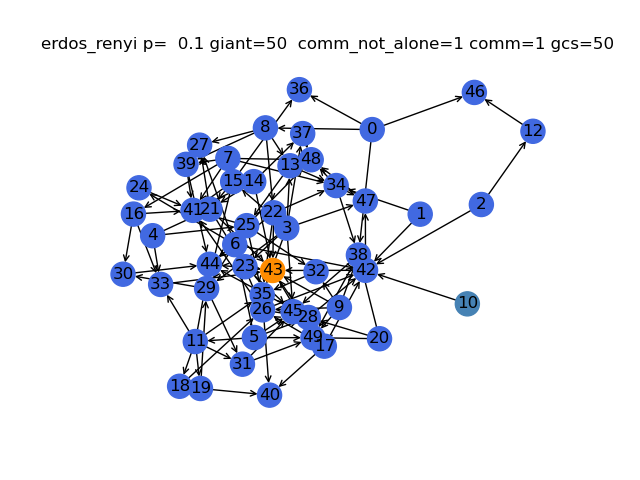
\includegraphics[width=0.5\linewidth]{with_directions.png}
    \caption{Similar to Erdös–Rényi of \ref{fig:no_directions} but with incoming links representing the banks which could be borrowing from each bank}
    \label{fig:with_directions}
\end{figure}

Either these links are generated in advance of the shock, they are potential agreements that can or cannot correspond to the real necessities of banks.

\subsection*{Trading strategy}

We assume that banks are risk-neutral agents operating in a perfect competition environment to optimize their expected profit. The expected profit of the bank $i$ for a loan provided to $j$ is given by

\begin{equation}
\mathbb{E}[\Pi_t^{i,j}] = \underbrace { p_t^j (r_t^{i,j} c_t^{i,j}) }_{\text{normally pays}}+ \underbrace {(1 - p_t^j)(\xi A_t^j - c_t^{i,j})}_{\text{when fails}} + \underbrace {\phi A_t^j - \chi A_t^i}_{\text{screening costs}}
\label{eq:expected_profit}
\end{equation}

where $A^i_t=C^i_t+L^i_t+R^i_t$ are the assets of the lender $i$ (as equal to $A^j_t$ of the borrower $j$), and $p^j_t$ is the probability that the borrower will not fail (probability of surviving),
$r^{i,j}_t$ the interest rate asked by the lender $i$ to the
borrower $j$, $c^{i,j}_t$ the maximum amount $i$ is willing
to lend to $j$. Moreover, $\xi$ is the liquidation cost of
assets, $A^j_t$, pledged as collateral, and $\phi$ and $\chi$ are the screening costs of creating a credit link that decrease with the dimension of the debtor and increase with the size of the creditor, defined in this case as  $\phi=0.025$ and $\chi=0.015$. In addition, we have a constant $\xi$ which is the collateral liquidation cost, and in our case we will use $\xi=0.3$.
Recalling that the borrower fails if its equity becomes negative $E^j_t<0$, the probability of surviving is given by the closeness between the' equity of $j$ and the highest net worth in the system:

\begin{equation}
\begin{aligned}[t]
 p^j_t=\frac{E^j_t}{E^{max}_t}
\end{aligned}
\quad\quad\quad\quad
\begin{aligned}[t]
 {p_{b}}^j_t=1-p^t_j=1-\frac{E^j_t}{E^{max}_t}
\end{aligned}
\label{eq:prob_surviving}
\end{equation}

Analogously, we can define the probability of bankruptcy as the opposite, also denoted in \ref{eq:prob_surviving} as $p_b$. The probability of surviving the bank is connected to financial fragility. A financial institution leaves the system if her net worth is so low that an adverse shock makes it negative or if she suffers a loss
so huge as to deplete all the net worth accumulated in the past. Finally, the maximum amount that the lender $i$ is willing to lend to $j$, that is the lending capacity is defined as

\begin{equation}
c_t^{i,j} = \begin{cases}
(1 - h_t^j) A_t^j > 0, & \text{if } (i,j) \in V_t, \\
0, & \text{otherwise}
\end{cases}
\label{eq:credit_constraint}
\end{equation}

where the borrower haircut is $h^j_t \in (0,h^{max}_t)$, defined as the $j$'s leverage, $\lambda^j_t $ with respect to the maximum one. so, $h^j_t=\frac{\lambda^j_t}{\lambda^{max}_t}$. 

The last component we will introduce is the power market $\psi$. It represents a market power parameter for lenders that captures their bargaining position ($\psi=0$) or monopolistic power ($\psi=1$) in our market:

\begin{itemize}
  \item $\psi = 0$: Competitive level (no lender power). The loan rate is the “fair” or actuarially competitive rate.
  \item $0 < \psi < 1$: Partial monopolistic power
  \item $\psi = 1$: Monopoly. Lenders use market power (e.g., limited competition, switching costs, informational advantages) to inflate the rate above this competitive benchmark, proportionally to a double in the competitive level (1+$\psi$).

\end{itemize}

This parameter $\psi$ captures information asymmetries (lenders' advantage over borrowers in a non-competitive market) or the opposite desired situation with no lenders charging high rates and borrowers easily switching lenders because there are many connections.

With all these components, and doing equal to zero the expected profit in \ref{eq:expected_profit}:


\begin{align*}
\mathbb{E}[\Pi_t^{i,j}] =  p_t^j (r_t^{i,j} c_t^{i,j}) &+ (1 - p_t^j)(\xi A_t^j - c_t^{i,j})+ \phi A_t^j - \chi A_t^i &= 0 \\
-p_t^j r_t^{i,j} c_t^{i,j} &=   (1 - p_t^j)(\xi A_t^j - c_t^{i,j})+ \phi A_t^j - \chi A_t^i  \\
r_t^{i,j} &= \frac{  (1 - p_t^j)(\xi A_t^j - c_t^{i,j})+ \phi A_t^j - \chi A_t^i}{-p_t^j c_t^{i,j}}  \\
r_t^{i,j} &= \frac{  -(1 - p_t^j)(\xi A_t^j - c_t^{i,j})- \phi A_t^j + \chi A_t^i}{p_t^j c_t^{i,j}}  \\
r_t^{i,j} &= \frac{ \chi A_t^i - \phi A_t^j -(1 - p_t^j)(\xi A_t^j - c_t^{i,j}) }{p_t^j c_t^{i,j}}  \\
\end{align*}
\label{eq:profits_equal_zero}

We can have the interest rate formula as

\begin{equation}
r_t^{i,j} = \underbrace{\frac{\chi A_t^i - \phi A_t^j - (1 - p_t^j)(\xi A_t^j - c_t^{i,j})}{p_t^j c_t^{i,j}}}_{\text{competitive baseline}} \times \underbrace{(1 + \psi)}_{\text{lender markup}}
\label{eq:interest_rate_decomposed}
\end{equation}

Consistent with asymmetric information and costly state verification \cite{Bernanke1999}, interest rates are determined by the size of the lender (measured by assets) and the leverage of the borrower. The budget identity underpins this pricing mechanism.


\subsection*{Equity evolution}


The next day, the repayment round takes place. Financial institutions encounter a new deposit movement that increases or decreases their liquidity once again \ref{evolution_d}. 
A new change in deposits face the banks to be able to pay the previous loan with the new income (positive shock after an initial negative), have a new opportunity to borrow the extra earns or directly bankruptcy if after the fire-sale process long term assets can not cover the debts in the worst scenario (negative shock after another previous negative one):

\begin{itemize}
\item If the borrower has a positive shock the liquidity could repay both principal and the interest
\item If the positive shock has not enough impact in deposits or if it is a negative shock, the borrower must sell its long-term assets to pay the principal, the interest and also the possible new negative variation in deposits, or fail if the long-term assets are not enough to pay the obligations, generating a bad debt in each lender bank $i$ due to the borrower $j$ noticed as $B^{i,j}_t$.
\item If the borrower $j$ pays to lender $i$ the loan correctly loan $l^{i,j}$, it generates earns at the interest rate $r^{i,j}$, so the equity of each bank evolves as ($\theta$ is the subset of failed banks and $\hat{L}$ the fire sales):
\end{itemize}


Banks that are failing affect creditors, as the law of motion of their equity is:

\begin{equation}
    E_t^i = E_{t-1}^i + \underbrace{ \sum_{j} l_{t-1}^{i,j} r_{t-1}^{i,j} }_{\text{repayment}}- \underbrace {\sum_{j \subseteq \theta_t^i} B_t^{i,j} - (1 - \rho) \tilde{L}_t^i}_{\text{bad debt}}
\label{eq:bank_equity}
\end{equation}

where we add to the equity of each bank the repayments of returned loans, using the specific interest rate $r^{i,j}$ for each granted loan $l^{i,j}$. And we subtract from the equity the bad debt generated by failed banks $j \subseteq \theta_t^i$ except the amount recovered by the fire sales.
Banks that cannot repay the principal and interest in full or cover their necessities also doing fire sales, exit the market ($E^i_t<0$). Banks exiting in $t$ are replaced in $t+1$ by the same number of entrants as outgoings, Entrants' size is small, as the initial values are used for these incumbents.


\begin{table}[h!]
\centering
\caption{Constants used in the simulations}
\begin{tabular}{cll}
\hline
\textbf{Constant} & \textbf{Value} & \textbf{Description} \\ 
\hline
$\mu$ & 0.7 & Shock parameters for perfect balance \\
$\omega$ & 0.55 &  \\
$\Phi$ & 0.025 & Screening costs \\
$\chi$ & 0.015 &  \\
$\xi$ & 0.3 & Liquidation cost of collateral \\
$\rho$ & 0.3 &  Fire sale cost \\
$\beta$ & 5 & Beta intensity of breaking the connection\\
$\alpha$ & 0.1 & Minimum value of  $E$ o $D$ before going into bankruptcy\\
$L_{i_0}$ &120  & Long term assets initial value \\
$C_{i_0}$ & 30  & Initial Capital.\\
& &  After reserves estimation it will be 27.3 (as $R_{i_0}=2.7)$\\
$D_i0$ & 135 & Initial Deposits value for each firm \\
$E_i0$ & 15  & Initial Equity initial\\
$r_i0$ & 0.02 & Initial rate \\
\hline
\end{tabular}
\end{table}

\newpage

\begin{figure}
\vspace{-3cm}
  \caption{Schema of the algorithm used in the model. Grey boxes are statistics obtained from the model in each step.}
  \label{fig:algorithm_figure}

%\begin{figure}
%\vspace{-3cm}
%  \caption{Schema of the algorithm used in the model. Grey boxes are statistics obtained from the model in each step.}
%  \label{fig:diagram}
%\end{figure}

\begin{tikzpicture}[
remember picture, overlay,
  node distance=1cm and 1cm,
  >=Stealth,
  trap/.style={
    trapezium,
    draw,
    trapezium left angle=-70,
    trapezium right angle=-110,
    minimum width=4cm,
    minimum height=1.5cm,
    align=center,
    font=\small,
    inner sep=8pt
  },
  every node/.style={font=\small},
  block/.style={rectangle, draw, rounded corners, align=center, minimum width=3cm, minimum height=1cm},
  decision/.style={diamond, draw, aspect=2, align=center},
  terminator/.style={ellipse, draw, align=center
 },
 textnode/.style={rectangle, align=left, minimum width=2.5cm, minimum height=0.8cm, font=\footnotesize},
 statistics/.style={rectangle, fill=lightgray!30, align=center, minimum width=1.5cm, minimum height=0.4cm, font=\scriptsize\ttfamily},
 iterate/.style={isosceles triangle,
  isosceles triangle apex angle=20,
  draw,aspect=2,
  fill=gray!5,
  shape border rotate=0,
  font=\small,
  align=center},
 decision/.style={diamond,
  draw,
  aspect=2.5, shape border rotate=0,
  minimum height=1cm,
  minimum width=1cm,
  inner sep=3pt,
  font=\small,
  align=center}
]
\begin{scope}[shift={(current page)}, xshift=-6cm, yshift=10.5cm]
\node[terminator] (start) {
  \texttt{model.initialize()} };
\node[iterate, below=0.7cm of start] (sim) {
  \texttt{model.simulate\_full()} \\$\forall t=0..T$};
\node[block, below=0.7cm of sim] (init) {
  \texttt{initialize\_step()}  };
\node[block, below=0.3cm of init] (links) {
  \texttt{setup\_links()} };
\node[block, below=0.3cm of links] (shock1) {
  \texttt{do\_shock("shock1")}  };
\node[block, below=of shock1] (ir) {
  \texttt{do\_interest\_rate()} };
\node[block, below=2cm of ir] (loans) {
  \texttt{do\_loans()} };
\node[block, below=3cm of loans] (shock2) {
  \texttt{do\_shock("shock2")} };
\node[block, below=of shock2] (repayments) {
  \texttt{do\_repayments()} };
\node[terminator, right=of sim] (finish) {
  \texttt{model.finish()} };

\node[statistics, right=0cm of links] (links_stats) {
  communities gcs \\
  communities\_not\_alone \\
  grade\_avg };

\node[statistics, anchor=north east, at=(shock1.south)] (shock1_stats) {
  incrD1  };

\node[statistics, anchor=north east, at=(shock2.south)] (shock2_stats) {
  incrD2 \\
  incrD };

\node[statistics, anchor=north east, at=(loans.south)] (loans_stats1) {
  psi\_effective \\
  active\_lenders \\
  active\_borrowers};

\node[statistics, right=0cm of loans_stats1] (loans_stats2) {
  sum\_loans num\_loans leverage\\
  equity\_lenders ir\_effective\\
  systemic\_leverage
};

\node[statistics, right=0cm of loans_stats2, yshift=-0.1cm] (loans_stats3) {
  num\_of\_rationed \\
  rationing };

\node[statistics, anchor=north east, at=(repayments.south)] (repayments_stats1) {
  liquidity equity  \\
  deposits bad\_debt \\
  profits reserves };

\node[statistics, right=0cm of repayments_stats1] (repayments_stats2) {
  best\_lender \\
  best\_lender\_clients };

\node[statistics, below=0cm of repayments_stats1, xshift=-1.5cm] (repayments_stats3) {
  potential\_credit\_channels \\
  bankruptcies \\
  bankruptcy\_rationed };

\node[statistics, below=0cm of repayments_stats3] (repayments_stats4) {
  prob\_bankruptcy \\
  c num\_banks maxE };

\node[statistics, anchor=north east, at=(ir.south)] (ir_stats) {
  asset\_i asset\_j \\
  ir psi \\
  potential\_lenders};


\node[textnode, right=of start] (start_text) {
  Initial conditions for each bank $r^i_0=0.02$:
    \begin{tabular}{l|l}
        \multicolumn{1}{c|}{\textbf{Assets}} &  \multicolumn{1}{c}{\textbf{Liabilities}} \\ \hline
        $C^i_0= 30-2.7 = 27.3$ &  $D^i_0= 135$\\
        $L^i_0= 120$  & $E^i_0= 15$ \\
        $R= 0.02 D^i_0 = 2.7$  &
    \end{tabular}  };


\node[textnode, right=of init] (init_text) {
    $bank.B=0$ \\
    $bank.rationing=0$ \\
    $bank.active\_borrowers=0 ... $
    };

\node[textnode, right=of links, xshift=2cm] (links_text) {
    Using Barabási–Albert graph of $m$ edges or \\
    Erdös-Rényi graph with probability of attachment $p_a$.};


\node[textnode, right=of shock1] (shock1_text) {
  $ D^i_t = D^i_{t-1} \left( \mu + \omega U(0,1) \right )$
 \\
  borrower if $\Delta D^i_t+C^i_t \le 0$ with demand $d=\Delta D$
  \\
  lender if $\Delta D^i_t+C^i_t > 0$ with supply $s= C +\Delta D$
 };



\node[textnode, right=of shock1_text] (shock2_text) {
    \begin{tabular}{l|l}
        \multicolumn{1}{c|}{\textbf{Lender}} &  \multicolumn{1}{c}{\textbf{Liab.}} \\ \hline
        $C^i_t\uparrow$ &  $D^i_t$\\
        $L^i_t$         & $E^i_t$ \\
        $R^i_t\uparrow$ &
    \end{tabular}

    \begin{tabular}{l|l}
        \multicolumn{1}{c|}{\textbf{Borrower}} &  \multicolumn{1}{c}{\textbf{Liab.}} \\ \hline
        $C^i_t \downarrow$ &  $D^i_t$\\
        $L^i_t$         & $E^i_t$ \\
        $R^i_t \downarrow$ & $d$
    \end{tabular}

};

\node[decision, right=of loans] (loans_text1) {
  $bank.d>0$? };



\node[textnode, below=of loans_text1] (loans_text5) {
    \begin{tabular}{l|l}
        \multicolumn{1}{c|}{\textbf{Lender}} &  \multicolumn{1}{c}{\textbf{Liab.}} \\ \hline
        $C^i_t$ &  $D^i_t$\\
        $L^i_t$  & $E^i_t$ \\
        $R^i_t$  & \\
        $s$ &
    \end{tabular}
    \begin{tabular}{l|l}
        \multicolumn{1}{c|}{\textbf{Borrower}} &  \multicolumn{1}{c}{\textbf{Liab}} \\ \hline
        $C^i_t$ &  $D^i_t$\\
        $L^i_t$  & $E^i_t$ \\
        $R^i_t$  & $l$ \\
    \end{tabular} };

\node[decision, right=of loans_text1] (loans_text2) {
  $bank.d \le lender.s$? };
\node[block, right=of loans_text2] (loans_text3) {
  \texttt{do\_firesales()}};

\node[block, below=0.3cm of loans_text3] (loans_text4) {
  Obtain loan};

\draw[->] (loans) -- (loans_text1);
\draw[->] (loans_text1) -- node[above, font=\scriptsize] {Yes: it's borrower}  (loans_text2);
\draw[->] (loans_text1.north) -- ++(0,0.4) node[above, font=\scriptsize]{No: it's lender} --   ++ (-3,0) --   (loans);
\draw[->] (loans_text2) -- node[above, font=\scriptsize] {No}  (loans_text3);
\draw[->] (loans_text2) -- node[above, font=\scriptsize] {Yes}  (loans_text4);
\draw[->] (loans_text3) --  (loans_text4);
% \draw[->] (loans_text4.west) -- ++(-1,0) |- ++(0,1.1) -- (loans);

\node[textnode, right=of shock2] (shock2__text1) {
  $ D^i_t = D^i_{t-1} \left( \mu + \omega U(0,1) \right )$
 };


\node[textnode, right=of shock2__text1] (shock2__text2) {
   \begin{tabular}{l|l}
        \multicolumn{1}{c|}{\textbf{Assets}} &  \multicolumn{1}{c}{\textbf{Liab.}} \\ \hline
        $C^i_t \uparrow$ if $\Delta D>0$&  $D^i_t$\\
        $L^i_t$  & $E^i_t$ \\
        $R^i_t \uparrow$ if $\Delta D>0$  & $d$ if $\Delta D<0$
   \end{tabular}  };


\node[decision, right=0.3cm of repayments] (repayments_text1) {
  $bank.l>0$? };
\node[decision, right=2cm of repayments_text1] (repayments_text2) {
  $loan+interest>C$? };
\node[block, right=1cm of repayments_text2] (repayments_text3) {
  \texttt{do\_firesales()}};
\node[decision, below=0.4cm of repayments_text2] (repayments_text4) {
  $bank.d>0$?};


\node[textnode, left=0.1cm of repayments_text4] (repayments_text7) { \\
Equity lender (prev. + loans - bad debt + firesales recovered): \\
$E_t^i = E_{t-1}^i + \sum_{j} l_{t-1}^{i,j} r_{t-1}^{i,j} - \sum_{j \subseteq \theta_t^i} B_t^{i,j} - (1 - \rho) \tilde{L}_t^i$
    };


\node[textnode, below=0.1cm of repayments_text7, xshift=-1.3cm] (repayments_text8) { \\
    \begin{tabular}{l|l}
        \multicolumn{1}{c|}{\textbf{Lender}} &  \multicolumn{1}{c}{\textbf{Liab.}} \\ \hline
        $C^i_t \uparrow$ &  $D^i_t$\\
        $L^i_t$  & $E^i_t  \uparrow$  \\
        $R^i_t \uparrow$
    \end{tabular}
    \begin{tabular}{l|l}
        \multicolumn{1}{c|}{\textbf{Borrower}} &  \multicolumn{1}{c}{\textbf{Liab.}} \\ \hline
        $C^i_t \downarrow$ &  $D^i_t$\\
        $L^i_t$  & $E^i_t  \downarrow$ \\
        $R^i_t \downarrow$
    \end{tabular}  };



\node[decision, below=0.2cm of repayments_text4] (repayments_text5) {
  $bank.failed$?};
\node[block, right=0.4cm of repayments_text5] (repayments_text6) {
  \texttt{replace\_bank()}};


\draw[->] (repayments) -- (repayments_text1);
\draw[->] (repayments_text1) -- node[above, font=\scriptsize] {Yes: borrower}  (repayments_text2);
\draw[->] (repayments_text1) -- node[above, font=\scriptsize] {No: lender}  (repayments_text4);
\draw[->] (repayments_text2) -- node[above, font=\scriptsize] {No} (repayments_text4);
\draw[->] (repayments_text2) -- node[above, font=\scriptsize] {Yes}  (repayments_text3);
\draw[->] (repayments_text4) -- node[right, font=\scriptsize] {Yes: shock2 negative and no capital}  (repayments_text3);
\draw[->] (repayments_text4) -- node[below, font=\scriptsize] {No}  (repayments_text5);
\draw[->] (repayments_text5) -- node[below, font=\scriptsize] {Yes}  (repayments_text6);


\node[textnode, right=0.3cm of ir] (ir_text1) {
  \quad \quad \quad \quad \quad \quad  $p_t^j=\frac{E^j_t}{E^{max}_t}$ \\
  $c^{i,j}_t=(1-h^i_j)A^j_t > 0$, if $(i,j) \in V_t$ \\
  $c^{i,j}_t=0$, otherwise \\
  $h^j_t=\frac{\lambda^j_t}{\lambda^{max}_t} $ \quad \quad \quad \quad
  $\lambda ^j_t=\frac{L^j_t}{E^j_t}$
 };
\node[textnode, right=0.3cm of ir_text1] (ir_text2) {
  $r_t^{i,j} = \frac{\chi A_t^i - \phi A_t^j - (1 - p_t^j)(\xi A_t^j - c_t^{i,j})}{p_t^j c_t^{i,j}} (1 + \psi)$
 };
\draw[->] (ir) -- (ir_text1);
\draw[->, shorten >=1pt, shorten <=1pt] (ir_text1) -- (ir_text2);





\draw[->] (start) -- (sim);
\draw[->] (sim) -- (init);
\draw[->] (init) -- (links);
\draw[->] (links) -- (shock1);
\draw[->] (shock1) -- (ir);
\draw[->] (ir) -- (loans);
\draw[->] (loans) -- (shock2);
\draw[->] (shock2) -- (repayments);
\draw[->] (sim.east) -- (finish);
\draw[->] (repayments.south) |- ++(0,-1) -- ++(-3,0) |- (sim.west);

\end{scope}
\end{tikzpicture}

\end{figure}
\;
\newpage

%\begin{equation}
%r_t^{i,j} = \frac{\chi A_t^i - \phi A_t^j - %(1 - p_t^j)(\xi A_t^j - c_t^{i,j})}{p_t^j c_t^{i,j}} {(1 + \psi)}
%\label{eq:interest_rate_decomposed1}
%\end{equation}

\bibliographystyle{plain}
\bibliography{paper}

\end{document}
